\documentclass[10pt]{article}
\usepackage[verbose, a4paper, hmargin=2.5cm, vmargin=2.5cm]{geometry}

\usepackage{fontspec}
\usepackage{ctex}
\usepackage{paratype}

\usepackage{amsmath}
\usepackage{amssymb}
\usepackage{amsfonts}
\usepackage{esint}
\usepackage{stmaryrd}

\usepackage[mathbf=sym]{unicode-math}
\setmainfont{STIX Two Text}
\setmathfont{STIX Two Math}

\setsansfont{Arial}
\setmonofont{Courier New}

\usepackage{makecell}
\usepackage{wasysym}
\usepackage{pifont}
\usepackage[export]{adjustbox}
\usepackage{graphicx}
\usepackage{mdframed}
\usepackage{booktabs,array,multirow}
\usepackage{tabularx}
\usepackage{hyperref}
\hypersetup{colorlinks=true, linkcolor=blue, filecolor=magenta, urlcolor=cyan,}
\urlstyle{same}
\usepackage[most]{tcolorbox}
\usepackage{tikz}

% 定义留白命令 - 用于教师板书
\newcommand{\boardspace}[1]{%
  \par\vspace{#1}
}

% 定义中难题留白（大幅留白供教师板书）
\newcommand{\hardboardspace}{%
  \par\vspace{5cm}
  \hfill\textit{（此处留白供课堂讲解）}
  \par\vspace{1cm}
}

% 定义大题留白
\newcommand{\largeboardspace}{%
  \par\vspace{8cm}
  \hfill\textit{（此处留白供课堂讲解与板书推导）}
  \par\vspace{1cm}
}

\definecolor{mygray}{RGB}{240,240,240}
\tcbset{
  colback=mygray,
  boxrule=0pt,
}
\graphicspath{ {./images/} }
\newcommand{\HRule}{\begin{center}\rule{0.9\linewidth}{0.2mm}\end{center}}
\newcommand{\customfootnote}[1]{
  \let\thefootnote\relax\footnotetext{#1}
}
\newcommand{\lt}{\mathrel{<}}
\newcommand{\gt}{\mathrel{>}}
\newcommand*\circled[1]{\tikz[baseline=(char.base)]{\node[shape=circle,draw,inner sep=1.5pt] (char) {\small #1};}}
\setcounter{MaxMatrixCols}{256}
\begin{document}
\begin{center}
\Large\textbf{2026届浦东新区高三下二模数学试卷}\\[0.5em]
\normalsize\textit{（学生版·课堂使用）}
\end{center}

\section*{一、填空题（第1-9题每题4分，第10-12题每题5分，共51分）}

1. 已知全集 \(U = \left( {0, + \infty }\right)\) ，集合 \(A = \lbrack 2, + \infty )\) ，则 \({\complement }_{U}A =\) \_\_\_\_.

\boardspace{1.5cm}

2. 若复数 \(z\) 满足 \(\left( {1 + \mathrm{i}}\right) z = {2\mathrm{i}}\) ，则复数 \(z =\) \_\_\_\_.

\boardspace{1.5cm}

3. 已知 \(f\left( x\right)  = \left\{  \begin{array}{l} \frac{1}{{x}^{3}},x < 0 \\  x + 1,x \geq  0 \end{array}\right.\) ,若 \(f\left( a\right)  =  - 2\) ，则实数 \(a\) 的值为\_\_\_\_.

\boardspace{1.5cm}

4. 在 \(\bigtriangleup  {ABC}\) 中，若 \(a = 7\) ， \(b = 8\) ， \(\cos C = \frac{13}{14}\) ，则 \(c =\) \_\_\_\_.

\boardspace{1.5cm}

5. 某校高中三年级 600 名学生参加了区质量检测,已知数学检测成绩 \(X\) 服从正态分布 \(N\left( {{100},{\sigma }^{2}}\right)\) (试卷满分为 150 分). 统计结果显示, 数学检测成绩介于 80 分到 120 分之间的人数为 450 名, 则此次检测中成绩不低于 120 分的学生人数约为总人数的\_\_\_\_(精确到 0.1\%).

\boardspace{1.5cm}

6. 已知直线 \(l\) 是曲线 \(y = \frac{3}{x + 1} + \ln x\) 在 \(x = 2\) 处的切线,则 \(l\) 的斜率为\_\_\_\_.

\boardspace{1.5cm}

7. 从 4 名男生 3 名女生中选取 3 人，依次进行面试，其中恰好有 1 名女生，则有\_\_\_\_种不同的面试方法.

\boardspace{1.5cm}

8. 一个家庭有两个孩子，生肖均为十二生肖之一(等可能). 已知其中一个孩子属马，则另一个孩子也属马的概率为\_\_\_\_.

\boardspace{1.5cm}

9. 已知数列 \(\left\{  {a}_{n}\right\}\) 的通项公式是 \({a}_{n} = {2}^{n - 1} + 1,{S}_{n}\) 为数列 \(\left\{  {a}_{n}\right\}\) 的前 \(n\) 项和,则使得不等式 \({S}_{n} > {2026}\) 成立的最小正整数 \(n\) 的值为\_\_\_\_.

\boardspace{1.5cm}

% 第10题开始为中难题，留足留白
10. 已知,圆 \(O\) 是圆心在原点的单位圆,弦 \({AB}\) 平行于 \(x\) 轴,并将圆分为两段弧. 将其中一段劣弧 \(\overset{\text{ ⏜ }}{AB}\) 沿弦 \({AB}\) 翻折后恰好经过圆心. 若直线 \(y = x + m\) 与翻折后得到的两段弧有四个不同的交点,则实数 \(m\) 的取值范围为\_\_\_\_.

\begin{center}
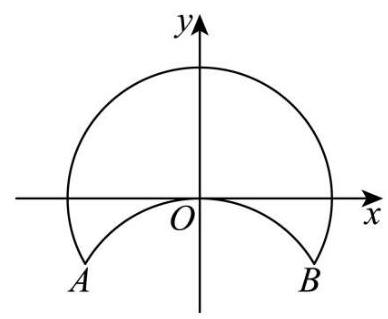
\includegraphics[max width=0.3\textwidth]{images/bo_d7ffgrqlb0pc73deo6k0_2_1121_1123_388_319_0.jpg}
\end{center}

\hardboardspace

11. 某光影科技实验室为长方体空间, 底面是边长为 4 米的正方形, 高为 3 米. 为营造动态光影效果, 在底面一个顶点处安装射灯 \(A\) ,在与该顶点相对的侧棱上、距底面 1 米处安装射灯 \(I\) ,两盖射灯的光束方向由智能系统自动控制，始终使两束光线相互垂直，且它们的交汇点 \(G\) 始终落在实验室天花板上，则交汇点 \(G\) 形成的轨迹长度为\_\_\_\_米.

\begin{center}
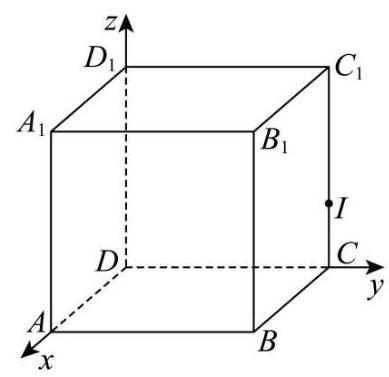
\includegraphics[max width=0.3\textwidth]{images/bo_d7ffgrqlb0pc73deo6k0_3_1106_539_389_377_0.jpg}
\end{center}

\hardboardspace

12. 已知集合 \(M\) 的元素均为正整数，定义集合 \(M\) 的"变项和"为:将 \(M\) 中每个元素 \(m\) 都乘以 \({\left( -1\right) }^{m}\) 后再求和. 若集合 \(A = \{ n \mid  1 \leq  n \leq  {2026},n \in  \mathbf{N}\}\) ，则集合 \(A\) 的所有非空子集的"变项和"的总和为\_\_\_\_.

\hardboardspace

\section*{二、单选题（每题5分，共20分）}

13. 某校学生会体育部长依据本校高三男生的身高(单位:cm)与体重(单位:kg)的抽样数据，运用电子办公软件求出了"体重"(y)关于"身高"(x)的回归方程，则该回归方程()

身高体重

174 55

176 58

176 62

181 74

182 88

179 68

169 54

168 52

171 56

180 86

\begin{center}
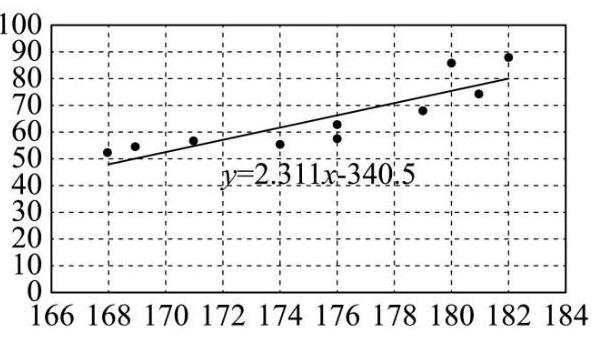
\includegraphics[max width=0.5\textwidth]{images/bo_d7ffgrqlb0pc73deo6k0_4_350_751_593_337_0.jpg}
\end{center}

A. 表示 \(x\) 与 \(y\) 之间的函数关系 B. 表示 \(x\) 与 \(y\) 之间的不确定关系

C. 反映 \(x\) 与 \(y\) 之间的真实关系 D. 反映 \(x\) 与 \(y\) 之间的真实关系的一种最佳拟合

\boardspace{2cm}

14. 已知实数 \(a,b,c\) 满足 \(a > b > 1 > c\) ,则下列结论一定正确的是( )

A. \({ac} > {bc}\) B. \({b}^{c} < 1\)

C. \({\log }_{a}b + {\log }_{b}a > 2\) D. \(a + c > b\)

\boardspace{2cm}

15. 已知 \(\overrightarrow{{e}_{1}},\overrightarrow{{e}_{2}}\) 与 \(\overrightarrow{{e}_{3}}\) 是不共面的向量,则以下向量组中,一定不共面的是 ( )

A. \(\overrightarrow{{e}_{1}} + \overrightarrow{{e}_{2}}\text{ 、 }\overrightarrow{{e}_{3}}\text{ 、 }\overrightarrow{{e}_{1}} + \overrightarrow{{e}_{2}} + \overrightarrow{{e}_{3}}\)

B. \(\overrightarrow{{e}_{1}}\text{ 、 }\overrightarrow{{e}_{2}} + \overrightarrow{{e}_{3}}\text{ 、 }3\overrightarrow{{e}_{1}} + 4\overrightarrow{{e}_{2}} + 3\overrightarrow{{e}_{3}}\)

C. \(\overrightarrow{{e}_{1}}\text{ 、 }2\overrightarrow{{e}_{2}} - \overrightarrow{{e}_{3}}\text{ 、 }\overrightarrow{{e}_{1}} - 2\overrightarrow{{e}_{2}} + \overrightarrow{{e}_{3}}\)

D. \(\overrightarrow{{e}_{1}} + \overrightarrow{{e}_{2}}\text{ 、 }\overrightarrow{{e}_{2}} + \overrightarrow{{e}_{3}}\text{ 、 }\overrightarrow{{e}_{1}} + k\overrightarrow{{e}_{3}}\) (其中 \(k\) 为实数)

\hardboardspace

16. 定义在 \(\mathbf{R}\) 上的非常值函数 \(y = f\left( x\right)\) ,若存在一个非零常数 \(T\) ,使得对任意 \(x \in  \mathbf{R}\) ,都有 \(f\left( {x + T}\right)  = T \cdot  f\left( x\right)\) 成立,那么称函数 \(y = f\left( x\right)\) 为 \(T\) 函数. 则下列说法正确的是( )

A. 存在函数 \(y = {kx} + b\left( {k \neq  0}\right)\) 为 \(T\) 函数

B. 若函数 \(y = f\left( x\right)\) 为 \(T\) 函数,且当 \(T > 1\) 时函数在 \(\lbrack 0,T)\) 上是严格增函数,则函数 \(y = f\left( x\right)\) 在 \(\lbrack 0, + \infty )\) 上是严格增函数

C. 若函数 \(y = f\left( x\right)\) 为 \(T\) 函数,且在 \(x = 0\) 处取得最小值,则 \(0 < T < 1\)

D. 若函数 \(y = f\left( x\right)\) 为 \(T\) 函数,且 \(\left| {f\left( x\right) }\right|  \leq  1\) 恒成立,则 \(y = f\left( x\right)\) 为周期函数

\hardboardspace

\section*{三、解答题（共79分）}

17. （14分）如图,在多面体 \({PQABCD}\) 中,平面 \({PAD} \bot\) 平面 \({ABCD},{AB}//{CD}//{PQ},{PD} \bot  {CD},\bigtriangleup {PAD}\) 是边长为 \(\sqrt{2}\) 的等边三角形, \({AB} = {PQ} = \frac{1}{2}{CD}\) .

\begin{center}
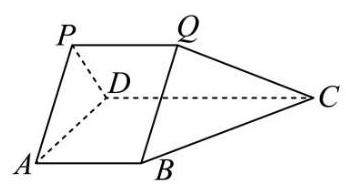
\includegraphics[max width=0.2\textwidth]{images/bo_d7ffgrqlb0pc73deo6k0_7_1158_1443_346_188_0.jpg}
\end{center}

(1)求证: \({AB}\bot\) 平面 \({PAD}\) ；

(2)若 \({PC}\) 与平面 \({ABCD}\) 所成的角为 \(\frac{\pi }{6}\) ，求多面体 \({PQABCD}\) 的体积.

\largeboardspace

\newpage

18. （14分）已知 \(f\left( x\right)  = \sqrt{3}\sin x + 2\cos \left( {x + \varphi }\right) ,\varphi  \in  \left\lbrack  {0,\pi }\right\rbrack\) .

(1)若函数 \(y = f\left( x\right)\) 是定义在 \(\mathrm{R}\) 上的奇函数，求常数 \(\varphi\) 的值；

(2)若 \(\varphi  = \frac{\pi }{3}\) ，若关于 \(x\) 的不等式 \(f\left( x\right)  + \frac{x}{2} - a > 0\) 对任意 \(x \in  \left\lbrack  {0,\pi }\right\rbrack\) 恒成立，求实数 \(a\) 的取值范围.

\largeboardspace

\newpage

19. （14分）某奶茶品牌为了解消费者对奶茶甜度的偏好情况, 随机抽取了 100 名顾客进行甜度测试 (分数越高表示越偏好甜味)、统计结果显示, 所有顾客的甜度偏好分数均分布在区间 \(\left\lbrack  {4,{10}}\right\rbrack\) 内,具体数据见下表:

\begin{center}
\adjustbox{max width=\textwidth}{
\begin{tabular}{|c|c|c|c|c|c|c|}
\hline
甜度偏好分数 & \(\lbrack 4,5)\) & \(\lbrack 5,6)\) & [6,7) & [7,8) & [8,9) & [9,10] \\
\cline{1-7}
人数 & 10 & 25 & 20 & 30 & 10 & 5 \\
\cline{1-7}
\hline
\end{tabular}
}
\end{center}

(1)估计该品牌奶茶消费者的平均甜度偏好分数(同一组数据用该区间的中点值作代表)；

(2)在这 100 名顾客中，用分层抽样的方法从甜度偏好分数在 \(\left\lbrack  {6,7}\right)\) 、 \(\left\lbrack  {7,8}\right)\) 这两组中共抽取 5 人. 再从这 5 人中随机抽取 3 人，记 \(X\) 为 3 人中甜度偏好分数在 \(\lbrack 7,8)\) 的人数，求 \(X\) 的分布、期望和方差；

(3)该奶茶品牌把甜度偏好分数在 \(\lbrack 7,9)\) 的消费者称"七分糖爱好者". 以样本估计总体、用频率代替概率，该品牌从某日消费人群中随机抽取 12 名消费者作为样本,记抽到 \(k\) 个"七分糖爱好者"的概率为 \({P}_{k}\) ,问当 \(k\) 为何值时 \({P}_{k}\) 最大?

\largeboardspace

\newpage

20. （18分）已知双曲线 \(C : {x}^{2} - \frac{{y}^{2}}{{b}^{2}} = 1\left( {b > 0}\right)\) 的左顶点为 \(A\) ,过点 \(D\left( {2,0}\right)\) 的直线 \(l\) 交双曲线 \(C\) 于 \(M\text{ 、 }N\) 两点,点 \(M\) 在第一象限.

(1)若双曲线 \(C\) 的焦距为 \(2\sqrt{5}\) ，求该双曲线 \(C\) 的离心率 \(e\) ；

(2)若 \(b = \sqrt{3}\) ， \(\bigtriangleup  {MAD}\) 为直角三角形，求点 \(M\) 的坐标；

(3)若双曲线 \(C\) 的一条渐近线方程为 \(x + \sqrt{2}y = 0\) ，点 \(M\) 、 \(N\) 均在双曲线 \(C\) 的右支，且存在实数 \(\lambda \left( {\lambda  < \frac{4}{3}}\right)\) ， 使得 \(\overrightarrow{MN} = \lambda \overrightarrow{MD}\) 成立,求直线 \(l\) 的倾斜角的取值范围.

\begin{center}
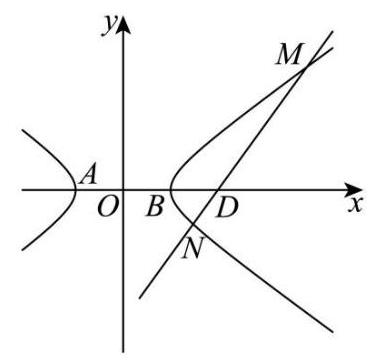
\includegraphics[max width=0.3\textwidth]{images/bo_d7ffgrqlb0pc73deo6k0_11_1145_1388_373_360_0.jpg}
\end{center}

\largeboardspace

\newpage

21. （19分）对于定义在区间 \(D\) 上的函数 \(y = f\left( x\right)\) ,定义集合 \(\Omega  = \left\{  {f\left( x\right) \begin{Vmatrix}{f\left( {x}_{1}\right)  - f\left( {x}_{2}\right) }\end{Vmatrix} \leq  \left| {{x}_{1} - {x}_{2}}\right| ,\forall {x}_{1},{x}_{2} \in  D}\right\}\) . 对任意闭区间 \(I \subseteq  D\) ,设函数 \(y = f\left( x\right)\) 在区间 \(I\) 上的最大值为 \({M}_{1}\) ,最小值为 \({M}_{2}\) ,记 \(M\left( {f,I}\right)  = {M}_{1} - {M}_{2}\) .

(1)若 \(f\left( x\right)  = {x}^{2} - x,D = \left\lbrack  {0,1}\right\rbrack\) ,判断函数 \(y = f\left( x\right)\) 是否属于集合 \(\Omega\) ,并求 \(M\left( {f,\left\lbrack  {0,1}\right\rbrack  }\right)\) 的值;

(2)若 \(D = \left\lbrack  {0,1}\right\rbrack  ,f\left( x\right)  \in  \Omega\) ,且 \(f\left( 0\right)  = 0,M\left( {f,\left\lbrack  {0,1}\right\rbrack  }\right)  = 1\) . 求 \(f\left( 1\right)\) 的值及函数 \(y = f\left( x\right)\) 的解析式;

(3)若 \(D = \lbrack 0, + \infty ),f\left( x\right)  \in  \Omega\) ,令 \(g\left( x\right)  = M\left( {f,\left\lbrack  {0,x}\right\rbrack  }\right)\) . 证明: \(y = f\left( x\right)\) 是单调函数的充要条件是: 对任意 \(0 < {x}_{1} < {x}_{2},\;g\left( {x}_{2}\right)  - g\left( {x}_{1}\right)  = M\left( {f,\left\lbrack  {{x}_{1},{x}_{2}}\right\rbrack  }\right)\) 恒成立.

\largeboardspace

\vfill
\begin{center}
\textit{— 试卷结束 —}
\end{center}

\end{document}
